\documentclass[10pt,letterpaper]{article}
\usepackage[margin=0.78in]{geometry}
\usepackage[T1]{fontenc}
\usepackage{lmodern,microtype,graphicx,booktabs,tabularx,amsmath,amssymb,xcolor,fancyhdr,enumitem}
\usepackage[hyphens]{url}
\usepackage[colorlinks=true,linkcolor=teal,urlcolor=teal]{hyperref}
\definecolor{ink}{HTML}{243447}\definecolor{teal}{HTML}{006B72}
\setlength{\parindent}{0pt}\setlength{\parskip}{6pt}\setlist{nosep,leftmargin=1.5em}
\pagestyle{fancy}\fancyhf{}\fancyhead[L]{\small Monthly means and reported temperature extremes}\fancyhead[R]{\small Independent study 32}\fancyfoot[C]{\thepage}\setlength{\headheight}{14pt}
\hypersetup{pdftitle={Monthly means and reported temperature extremes},pdfauthor={Independent research program},pdfsubject={Historical airport temperature aggregation, missing hourly slots and conditional year resampling}}
\begin{document}\color{ink}
{\LARGE\bfseries Monthly means and reported temperature extremes\par}
{\large Eight airport case studies for examining outdoor contingency scenarios\par}
\textbf{Independent research study 32}\hfill29 October 2026\\
AI-assisted analysis and manuscript. Not peer reviewed or accepted for formal publication.

\section*{Decision and verified finding}
A monthly outdoor-temperature mean cannot describe how often individual readings cross a planning threshold. A storage contingency scenario needs the distribution of relevant conditions, their missingness and a connection to the actual facility or product. This study examines the aggregation step in historical airport records; it does not validate a cold-chain system.

Across the eight fixed airports in the held descriptive years 2017--2024, there are 49,423 reported near-hour temperature slots strictly above the illustrative 30$^{\circ}$C threshold. Replacing every observed reading with its own observed monthly mean hides 26,642 of those positives, or 53.9\%. The same coarsened view labels 8,059 observed non-exceeding slots positive. This comparison uses the entire month's available readings and is not an out-of-sample forecast or an actual alert system.

\begin{center}\begin{tabularx}{\linewidth}{Xr}\toprule
Held reported-slot comparison, threshold 30$^{\circ}$C & Value\\\midrule
Reported temperature slots above threshold & 49,423\\
Positive slots hidden by their monthly mean & 26,642 (53.9\%)\\
Non-exceeding slots labeled positive by the monthly view & 8,059\\
Airports with every reported positive hidden & 6 / 8\\\bottomrule
\end{tabularx}\end{center}

\textbf{Missingness is a separate decision risk.} Minneapolis has 10,966 unknown slots in the held period, 15.6\% of its calendar grid. Its mean annual observed positive count is 110.75, but the conservative possible-count upper bound is 1,481.5. That range overlaps Dallas/Fort Worth's 1,279.5--1,282.25 bound. The recorded subset cannot establish their full-grid ordering. Unknown slots are retained rather than treated as cool conditions or dropped with a station.

\textbf{Practical recommendation.} Present threshold counts, observed coverage and explicit unknown-slot bounds alongside monthly means. Check the full quality-bearing source and measure the relevant facility environment before turning an outdoor scenario into a contingency choice. These results do not establish storage capacity, product failure, realized savings or a general city ranking.

\textbf{Limits of the measurement.} ISD-Lite provides selected observations near the top of an hour; counted positive slots do not prove that the temperature exceeded the threshold for every minute of an hour. Airport readings do not measure warehouse, vehicle or product temperatures. Lite omits the full quality flags and adds no further QC [3]; individual observation quality is unverified. The archive also carries a general merge notice [6]. Resampling reported years cannot resolve these limits or guarantee future climate coverage.

\clearpage
\section*{1. Fixed source panel and complete accounting}
We use NOAA's ISD-Lite product, the reduced hourly subset described by NCEI [1,3]. The official June 2026 service notice directs users to the NODD archive and states that ISD stopped updating after 24 August 2025 [2]. We therefore use completed years 2010--2024, not partial 2025, current conditions or the newer GHCNh product. Source access uses the published public bucket with no account or paid service.

Station-history identifiers and record periods were verified before measurement retrieval. Development is 2010--2016; held descriptive evaluation is 2017--2024. The eight stations were fixed for geographic variety as airport case studies, not sampled to represent all cities or selected from their temperature results. Each site has 131,496 expected UTC calendar slots across the full period, including leap-day hours.

\begin{center}\small\begin{tabular}{llrr}\toprule
Airport case & USAF / WBAN & Unknown, 2010--2024 & Unknown, held years\\\midrule
Atlanta & 722190/13874 & 79 & 67\\
Chicago O'Hare & 725300/94846 & 60 & 32\\
Dallas/Fort Worth & 722590/03927 & 26 & 22\\
Miami & 722020/12839 & 68 & 55\\
Minneapolis & 726580/14922 & 10,974 & 10,966\\
New York JFK & 744860/94789 & 30 & 24\\
Phoenix & 722780/23183 & 27 & 17\\
Seattle--Tacoma & 727930/24233 & 78 & 70\\
\bottomrule\end{tabular}\end{center}

The full capture contains 1,051,655 source rows in 120 station/year files. Of 1,051,968 expected calendar slots, 1,040,626 have a reported temperature, 11,029 have an explicit missing-temperature sentinel and 313 have no source row. Thus 11,342 slots are unknown. The held grid contains 561,024 expected slots, with 549,771 observed and 11,253 unknown. Every fixed station and year remains in the accounting; no completeness cutoff or station replacement was introduced.

Each ordinary source GET records its URL, retrieval time, compressed bytes, ETag, Last-Modified and SHA-256. All 120 objects pass a final ordinary HEAD consistency check. Compressed and decompressed payload hashes, every selected time/temperature field and its original line locator are independently reconciled. This establishes a bounded capture of the published records, not their historical availability for a forecast.

Only selected station/time/temperature facts, locators, hashes and original analysis are public. Full source files, agency documents and artwork remain outside Git. NODD's reuse terms request attribution and prohibit an implication of NOAA endorsement; this analysis is a derivative, not unchanged NOAA output [4]. Public airport metadata describes infrastructure, without passenger, private, clinical or product records.

\clearpage
\section*{2. Exact aggregation, unknown slots and protected sequence}
ISD-Lite selects observations in a documented window near the top of the hour and resolves duplicates within its parent data [3]. We parse the inherited UTC hour label and temperature in integer tenths of a degree Celsius; $-9999$ is missing. Dates, station/year identity and source-hour uniqueness must pass. A fixed broad sanity guard accepts nonmissing values from $-100.0$ to $70.0^{\circ}$C, without truncating or repairing a failure. This is a parser safeguard, not manual physical-weather validation. Full Lite quality flags are unavailable.

For a fixed station/year/month, let $n$ be the number of observed temperature slots, $s$ the sum of their integer-tenths temperatures and $e$ the count with $T>10u$. Thresholds $u=25,30,35^{\circ}$C are illustrative scenarios fixed before values; 30$^{\circ}$C is primary. They are not product-safety limits, manufacturer setpoints or optimized alert thresholds. Equality is non-exceeding.
\[
\overline T=\frac{s}{10n},\qquad
A=1(s>10un),\qquad
TP=Ae,\quad FP=A(n-e),\quad FN=(1-A)e,\quad TN=(1-A)(n-e).
\]
The monthly view labels all $n$ observed slots positive when their observed mean crosses the threshold. Empty observed months retain an undefined mean/classification; no artificial cold value is inserted. Precision, recall and hidden-positive fraction are exact rational quantities, undefined for zero denominators. All monthly and annual confusion counts are retained. The reference label is the reported reading, not a product state or an independently audited true temperature.

For a year with $H$ expected slots and $U=H-n$ unknown temperatures, positive-slot counts have conservative bounds $[e,e+U]$. These bounds concern the reported/unknown calendar grid. They are separate from sampling intervals and do not bound product exposure or true-weather measurement error. They also do not bound the hypothetical complete-month mean: unobserved temperatures could change that mean and its classification of observed slots.

Confirmed positive-slot runs break at an unknown slot; possible runs allow unknown slots to be positive and break at a confirmed nonpositive. Runs reset at each UTC year boundary. Their lengths are counts of consecutive hour labels, not demonstrated continuous physical duration. Empirical 95th/99th percentiles use nearest rank $\lceil pn\rceil$, with maxima and all year results retained. No extreme-value distribution, return level or rare-event forecast is fitted.

All-year source/schema/coverage/missing checks were visible and inputs were not blinded. Development analytical summaries ran before the public eighteen-dependency freeze at revision \texttt{9b72dd3}; held threshold, confusion, run, tail and resampling summaries ran afterward. There is no learned preprocessing, fitted model, cutoff optimization or seed search. This protects the computation sequence, without converting it into prospective climate validation.

\clearpage
\section*{3. Every airport in the primary held comparison}
The table shows all eight cases for the 30$^{\circ}$C scenario. Hidden percentage is $FN/e$ conditional on reported temperatures and means computed from the available readings. The last column averages each year's positive-count lower and upper bounds. It is not a confidence interval. Hidden percentages are rounded; the mean annual count bounds are exact to three decimals for eight years.

\begin{center}\small\setlength{\tabcolsep}{4pt}\begin{tabular}{lrrrrl}\toprule
Airport & Observed & Unknown & Positive & Hidden & Mean annual count bounds\\\midrule
Atlanta & 70,061 & 67 & 3,829 & 100.0\% & [478.625, 487.000]\\
Chicago O'Hare & 70,096 & 32 & 1,526 & 100.0\% & [190.750, 194.750]\\
Dallas/Fort Worth & 70,106 & 22 & 10,236 & 63.1\% & [1279.500, 1282.250]\\
Miami & 70,073 & 55 & 8,178 & 100.0\% & [1022.250, 1029.125]\\
Minneapolis & 59,162 & 10,966 & 886 & 100.0\% & [110.750, 1481.500]\\
New York JFK & 70,104 & 24 & 700 & 100.0\% & [87.500, 90.500]\\
Phoenix & 70,111 & 17 & 23,622 & 19.6\% & [2952.750, 2954.875]\\
Seattle--Tacoma & 70,058 & 70 & 446 & 100.0\% & [55.750, 64.500]\\
\bottomrule\end{tabular}\end{center}

\begin{center}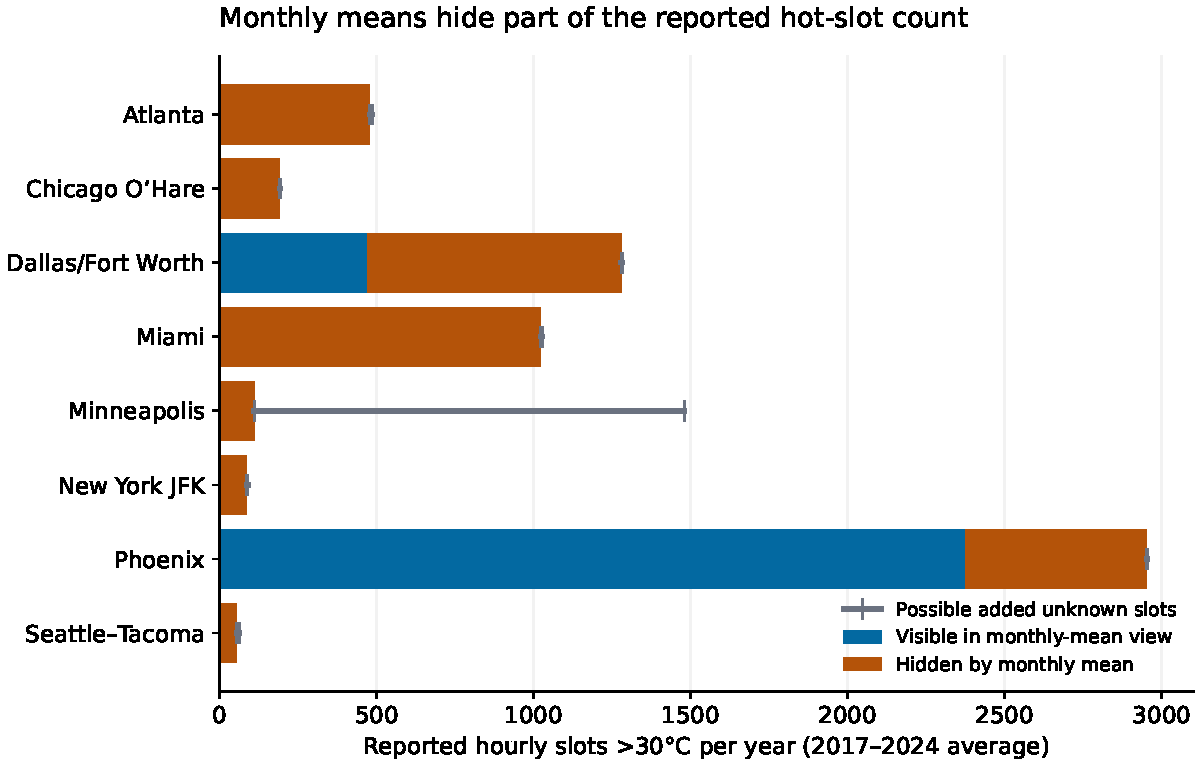
\includegraphics[width=\linewidth]{images/monthly_aggregation_gap.pdf}\end{center}
{\small\textbf{Figure 1.} Mean annual reported positive slots in 2017--2024, decomposed into those visible to the monthly-mean view (blue) and hidden by it (orange). Gray extensions show the possible added count if every unknown slot were positive. This is a common count axis, not an inferred full-city or facility exposure comparison. The large Minneapolis extension makes its missingness visible.}

Across the observed grid, $TP=22,781$, $FP=8,059$, $FN=26,642$ and $TN=492,289$. The monthly view labels 30,840 observed slots positive, compared with 49,423 individual reported positives; the net count gap differs from the hidden-positive count because false positives partially offset false negatives. No actual company's dashboard or alert behavior is asserted.

\clearpage
\section*{4. Seasonal detail and the meaning of the monthly view}
\begin{center}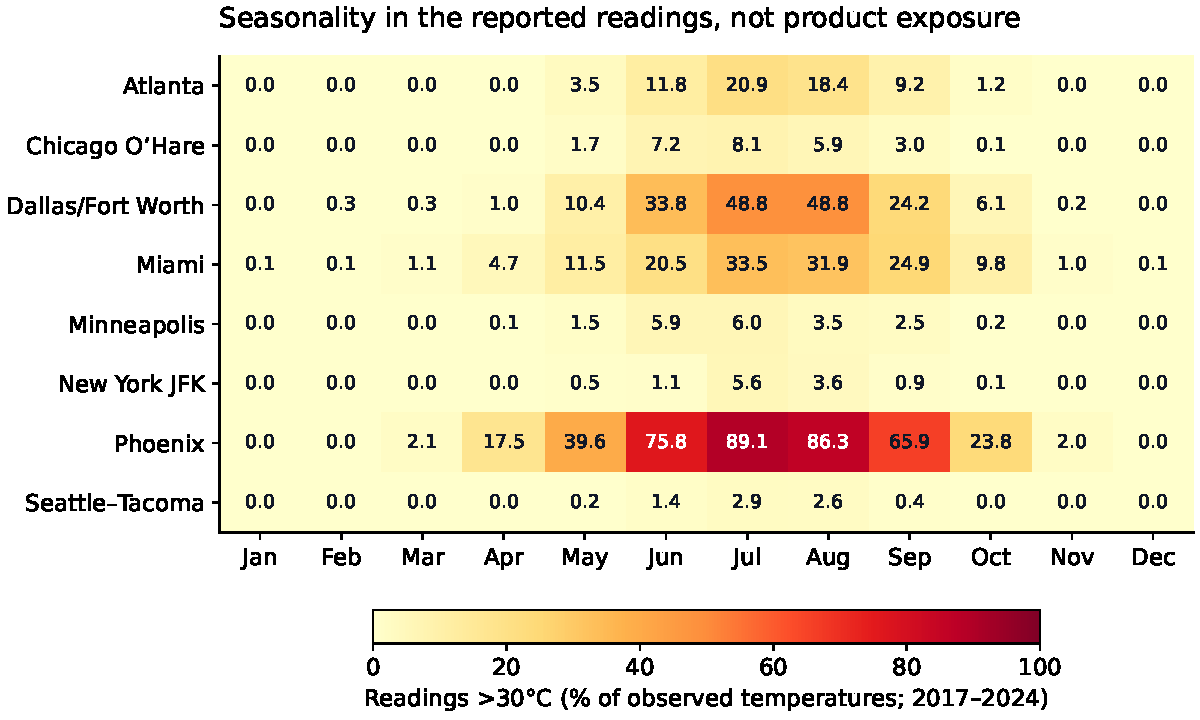
\includegraphics[width=\linewidth]{images/monthly_reported_tail.pdf}\end{center}
{\small\textbf{Figure 2.} For each airport and UTC calendar month, the percentage of observed held-year readings strictly above 30$^{\circ}$C. Each cell pools that calendar month across 2017--2024. The natural 0--100\% scale does not clip high values; cell labels retain one decimal. The denominator excludes unknown temperatures and is available in the complete monthly tables. This seasonal display is distinct from the classification calculation, which uses each individual year/month's mean.}

Phoenix has high reported positive fractions in its summer months, including 89.1\% in July. A monthly average can still hide individual positives near seasonal boundaries or at other thresholds. Conversely, a month with a mean above the threshold labels its non-exceeding readings positive in this coarsened comparison. The full confusion table preserves both effects instead of presenting only a favorable reduction in hidden counts.

Atlanta, Chicago, Miami, Minneapolis, New York JFK and Seattle--Tacoma have no observed monthly mean above 30$^{\circ}$C in the held panel, while each has reported readings above it. Dallas/Fort Worth and Phoenix have both visible and hidden positives. These are properties of the fixed records and observed means, not general assertions about every location or future year in those cities.

Missingness can be weather-dependent. In particular, a percentage of Minneapolis's observed readings is not a full-calendar climate rate. Unknown temperatures can change the count, the complete-month mean and which observed slots the coarsened view would label positive. The figure does not fill those gaps, infer a missing-data mechanism or remove the station.

The useful measurement lesson is to keep a mean and a threshold-frequency view together, with the denominator and time basis visible. An actual storage scenario additionally needs site measurements, facility response, backup behavior and the relevant product specifications. None is supplied by an outdoor airport archive.

\clearpage
\section*{5. Every threshold and conditional whole-year resampling}
\begin{center}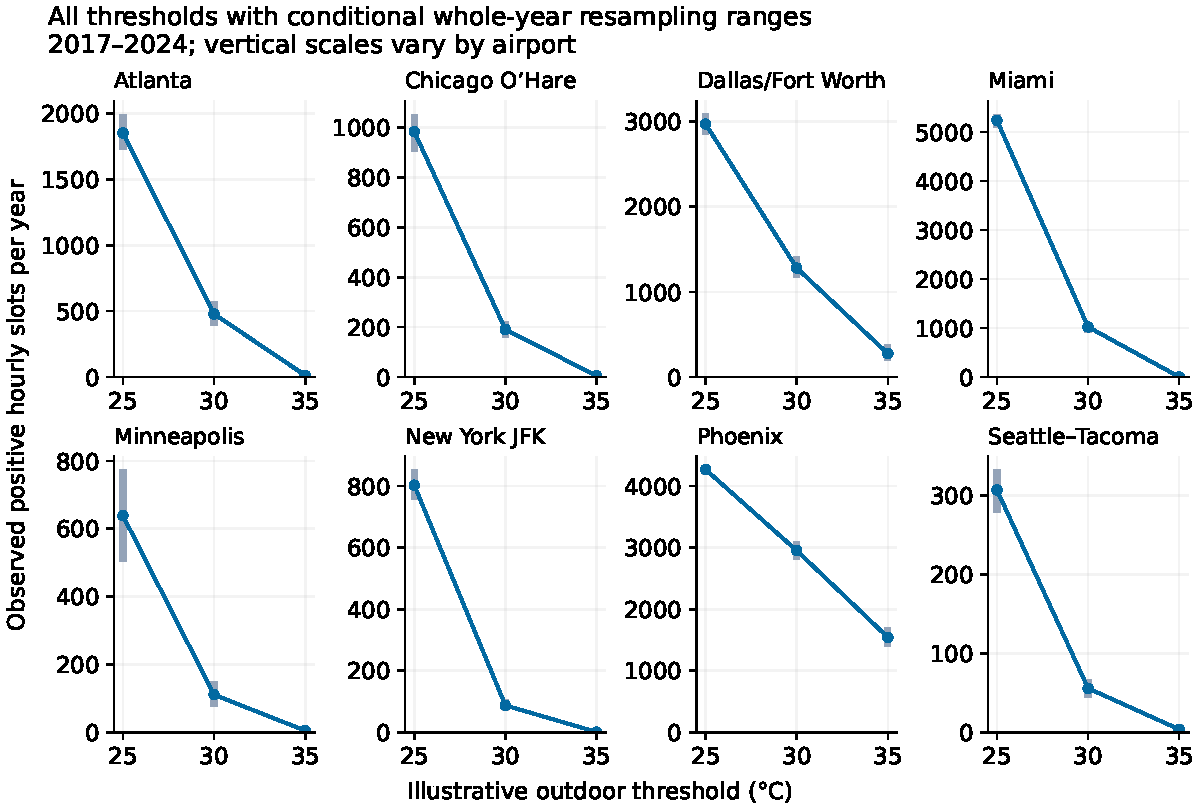
\includegraphics[width=\linewidth]{images/threshold_year_ranges.pdf}\end{center}
{\small\textbf{Figure 3.} All three fixed thresholds for every held airport. Blue points/lines are mean annual observed positive-slot counts; gray ranges are nominal 90\% whole-year resampling percentiles conditional on the recorded years. Vertical scales vary by airport and are labeled. These ranges do not include unobserved-temperature uncertainty or validate future-year coverage; the common-axis missing-slot bounds appear in Figure 1.}

For each phase, 500 draws resample whole years with replacement. The same year-index matrix is shared across all airports and thresholds, preserving within-year temporal structure and contemporaneous cross-airport patterns. NumPy's declared seed is 20261029. Held draws contain eight years; development draws contain seven. Each replicate mean is an exact fraction. Endpoints use ordered replicate positions 25 and 475, without interpolation.

\begin{center}\small\begin{tabular}{lrl}\toprule
Primary threshold, airport & Observed mean / year & Conditional 90\% resampling range\\\midrule
Atlanta & 478.625 & [389.125, 571.375]\\
Chicago O'Hare & 190.750 & [159.000, 222.500]\\
Dallas/Fort Worth & 1279.500 & [1166.125, 1413.875]\\
Miami & 1022.250 & [916.375, 1117.125]\\
Minneapolis & 110.750 & [75.000, 149.750]\\
New York JFK & 87.500 & [71.750, 105.375]\\
Phoenix & 2952.750 & [2808.125, 3095.500]\\
Seattle--Tacoma & 55.750 & [43.625, 67.000]\\
\bottomrule\end{tabular}\end{center}

These are exploratory conditional resampling ranges. They resample each year's observed count and its missingness pattern; they are not a correction for gaps. Year exchangeability, climate trends and dependence across years are unverified. No p-value, ranking probability, future-climate guarantee or operational benefit is inferred from a narrow range.

\clearpage
\section*{6. Missingness, empirical tails and sample runs}
Minneapolis's largest temperature gaps occur in 2020--2022: 3,666, 3,641 and 3,605 unknown slots respectively. The source still has rows for other meteorological fields in many such hours; a source-row count is therefore not the same as temperature coverage. We retain both absent rows and explicit missing temperatures. No claim about why these temperatures are missing is established.

\begin{center}\small\begin{tabular}{lrrrr}\toprule
Airport & Observed 99th percentile & Observed maximum & Confirmed run & Possible run\\
 & ($^{\circ}$C) & ($^{\circ}$C) & (slots) & (slots)\\\midrule
Atlanta & 33.3 & 37.2 & 15 & 15\\
Chicago O'Hare & 31.7 & 37.8 & 15 & 15\\
Dallas/Fort Worth & 37.8 & 42.8 & 45 & 45\\
Miami & 33.3 & 36.7 & 18 & 34\\
Minneapolis & 31.1 & 37.8 & 16 & 23\\
New York JFK & 30.0 & 36.7 & 16 & 16\\
Phoenix & 43.9 & 48.3 & 622 & 622\\
Seattle--Tacoma & 29.4 & 41.7 & 15 & 15\\
\bottomrule\end{tabular}\end{center}

These are pooled held reported-temperature tails and the largest annual 30$^{\circ}$C sample-run bounds. Miami's confirmed/possible run counts are 18 and 34; Minneapolis's are 16 and 23. Phoenix has 622 consecutive positive hour labels in its largest annual run. None proves an uninterrupted physical exposure of that many hours: observations between the selected readings, exact original minutes and product conditions are not available in Lite. Maxima and empirical percentiles also condition on observed readings and source quality; missing extreme values need not be captured.

The archive carries an undated general notice that some ISD merging can leave output unsorted or unmerged [6]. It does not identify these selected Lite files or certify an individual temperature as wrong. Selected station/hour uniqueness and independent source extraction pass, while individual observation QC remains unknown. The notice was read after the held arithmetic checks and documented separately; no station, source value, threshold, period or algorithm was changed in response. Arithmetic agreement cannot resolve physical-data quality.

\textbf{What the evidence supports.} The fixed source product exhibits a measurable difference between individual reported threshold readings and monthly aggregation, and a material missingness limitation in one case. It supports a reproducible measurement audit, with all results and caveats exposed. It does not identify how much cooling or redundancy a warehouse needs, predict product spoilage, establish city-wide conditions or constitute a future-climate risk assessment.

\textbf{Next evidence.} Obtain quality-bearing observations and review flagged/merged records; characterize local warehouse or vehicle temperatures, thermal response and backup duration; then define a product-specific, authorized scenario. Treat that as a separate study with its own evidence, rather than labeling this outdoor sample comparison as deployed cold-chain planning.

\clearpage
\section*{7. Reproduction and independent evidence}
The repository retains selected temperature facts, exact source/locator hashes, complete coverage, all three thresholds, every monthly/year/phase table, all resampled year indices and all 24,000 station/threshold replicate rows. The source certificate independently checks 5,258,275 selected source fields and 8,413,240 projected scalars, all 120 station-year coverage rows and eight station metadata rows. Full originals and documents remain outside Git.

Twelve boundary fixtures cover strict equality, missing sentinels, empty means, false positives/negatives, missing-breaking/bridging runs, leap hours, exact means, nearest-rank quantiles and invalid source years. Independent full calendars, SQLite grouped integer sums, SQL window-island run lengths and sorted order statistics reconstruct the results. Development/held checks verify 190,540 exact scalars and 66,840 reported floats, including every retained year-block draw and interval. Reported floats use a $10^{-12}$ numerical comparison tolerance; the substantive arithmetic remains integer/rational.

Isolated replay matches 330,561 CSV fields or JSON documents exactly and verifies eighteen frozen dependencies. All 200 plotted values are checked on actual artists. The heatmap's 96 annotation texts and 96 contrast pairs are checked, with a natural 0--100\% range; no accessibility conformance is inferred. Every rendered manuscript page and the approved publication bytes are checked separately, including bounded private-path/token and PDF active-content exclusions. Finite checks do not establish universal correctness or replace the source-quality limitations.

\begin{verbatim}
python -m pip install -r requirements.txt
python -m unittest discover -s tests -v
python src/check_reproduction.py
python src/verify_figures.py
python src/verify_paper.py
python src/verify_public_package.py
\end{verbatim}
Python 3.10; NumPy 2.2.5, Matplotlib 3.10.9 and pypdf 6.10.0. After dependency installation, these commands require no live source access or private originals. Publication state, exact candidate/main Linux runs, tree identity and the annotated tag are recorded by repository/program receipts; this manuscript does not presume a remote gate passed before verification.

\subsection*{Primary sources and dataset documentation}
{\footnotesize
[1] NOAA NCEI. \href{https://www.ncei.noaa.gov/products/land-based-station/integrated-surface-database}{Integrated Surface Database and ISD-Lite product description}.\par
[2] NOAA NESDIS, 23 June 2026. \href{https://www.nesdis.noaa.gov/news/service-location-change-integrated-surface-data-global-hourly}{Service-location change and cessation of ISD updates}.\par
[3] NOAA. \href{https://noaa-isd-pds.s3.amazonaws.com/isd-lite/isd-lite-format.txt}{ISD-Lite format}; \href{https://noaa-isd-pds.s3.amazonaws.com/isd-lite/isd-lite-technical-document.txt}{technical document}; \href{https://noaa-isd-pds.s3.amazonaws.com/isd-format-document.pdf}{original ISD format/UTC fields}.\par
[4] \href{https://registry.opendata.aws/noaa-isd/}{NOAA ISD NODD registry}: published public access, attribution and derivative/endorsement limits.\par
[5] NOAA. \href{https://noaa-isd-pds.s3.amazonaws.com/isd-history.csv}{Station-history metadata}; selected station/year object URLs and hashes are listed in the public source manifest. Access: 29 October 2026.\par
[6] NOAA archive. \href{https://noaa-isd-pds.s3.amazonaws.com/NOTICE-ISD-MERGE-ISSUE.TXT}{General ISD merge notice}, undated; applicability to specific selected Lite readings unverified.\par
}
\end{document}
